\section{Thống kê mô tả}

\subsection{Phân tích biến liên tục bằng biểu đồ.}
\subsubsection{Đồ thị Histogram}
	Vì nhóm làm phân tích các ảnh hướng đến chi phí đơn hàng nên sẽ không có customer\_lat và customer\_long. Dưới đây là một số hình ảnh của các biến order\_price, delivery\_charges, coupon\_dis-count, order\_total, distance\_to\_nearest\_warehouse. Khi biểu diễn bằng đồ thị Histogram
\begin{figure}[H]
    \centering
    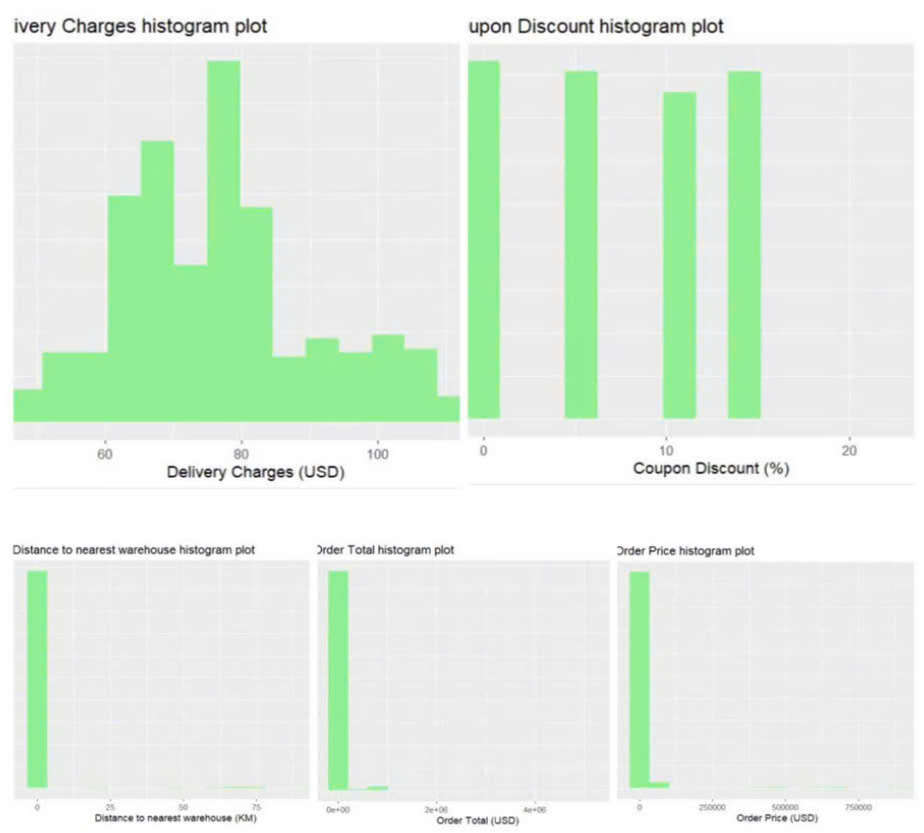
\includegraphics[width=0.7\linewidth]{graphics/bang7.jpg}
    \caption{Đồ thị Histogram của các biến liên tục}
\end{figure}
\FloatBarrier

\textbf{Nhận xét}: Ta nhận thấy rằng, từ kết quả đồ thị histogram cho thấy biến order\_total, order\_price, distance\_to\_nearest\_warehouse có phân phối lệch phải, với một cột cao ở phía bên trái. Điều này cho thấy hầu hết khách hàng chỉ chi tiêu ở mức thấp hơn, trong khi một số ít có tổng giá trị đơn hàng cao, tạo ra các điểm ngoại lệ. Phân phối lệch phải thường cho thấy  rằng có một số khách hang chi tiêu rất cao, điều này có thể ảnh hưởng đến quy mô hình hồi quy. Sau khi kiểm tra tỉ lệ khuyết nhỏ của các ngoại lai .Để xử lí tình trạng phân phối lệch phải này, ta áp dụng xóa bỏ các ngoại lai  của order\_total, order\_price, distance\_to\_nearest\_warehouse.


 Dưới đây là hình ảnh sau khi xóa ngoại lai.
 \begin{figure}[H]
    \centering
    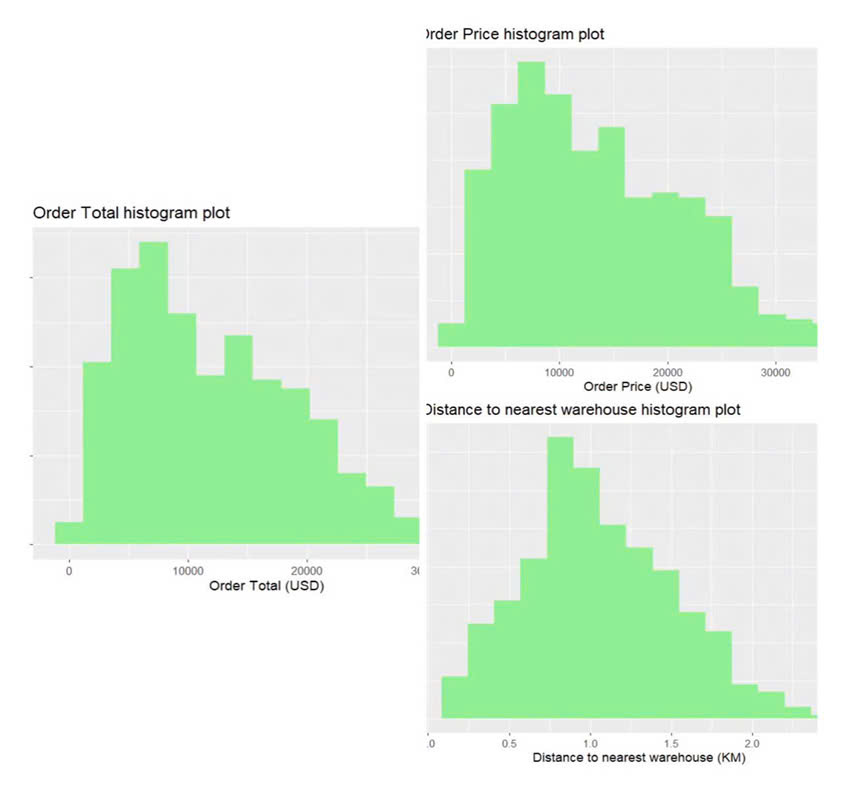
\includegraphics[width=0.7\linewidth]{graphics/bang8.jpg}
    \caption{Đồ thị Histogram của các biến liên tục đã xóa ngoại lai}
    
\end{figure}
\subsubsection{Đồ thị phân tán}
Ta so sánh  lần lượt từng order\_price, delivery\_charges, coupon\_discount, distance\_to\_nearest\_-warehouse với order\_total. Với những hình ảnh có những chấm màu xanh là chưa xóa ngoại lai, còn những hình có chấm màu đỏ là đã xóa ngoại lai.
\begin{figure}[!htbp]
    \centering
    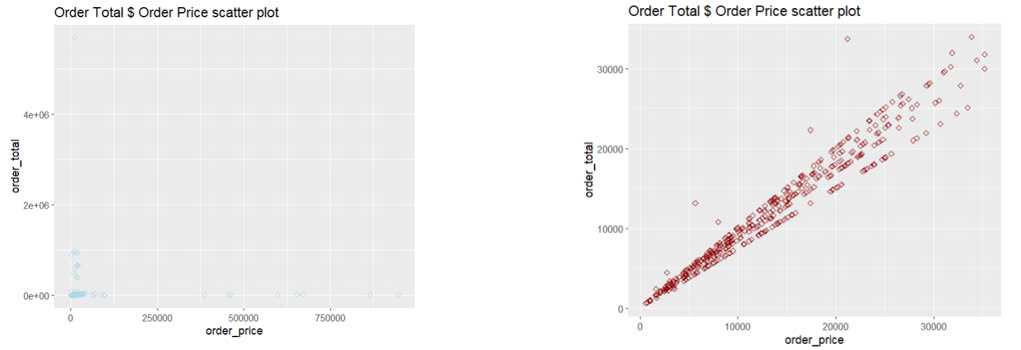
\includegraphics[width=0.8\linewidth]{graphics/bang9.jpg}
    \caption{Hình chưa xóa ngoại lai và đã xóa của order\_price}
 
\end{figure}
\begin{figure}[!htbp]
    \centering
    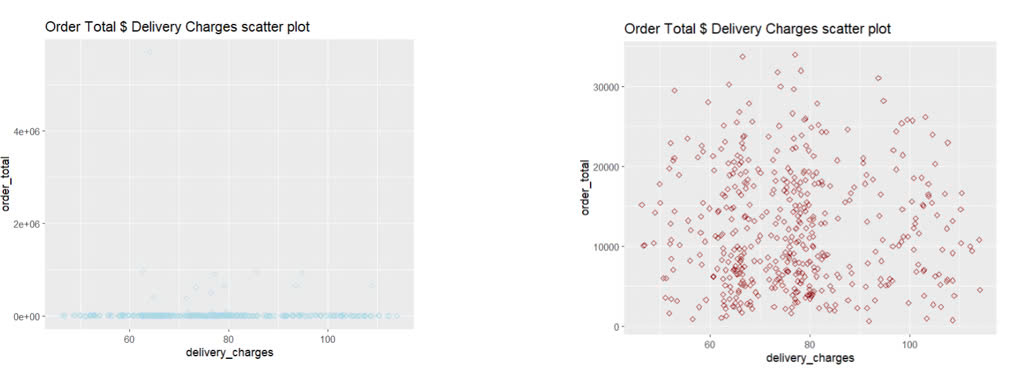
\includegraphics[width=0.8\linewidth]{graphics/bang10.jpg}
    \caption{Hình chưa xóa ngoại lai và đã xóa của delivery\_charges}
    
\end{figure}
\begin{figure}[!htbp]
    \centering
    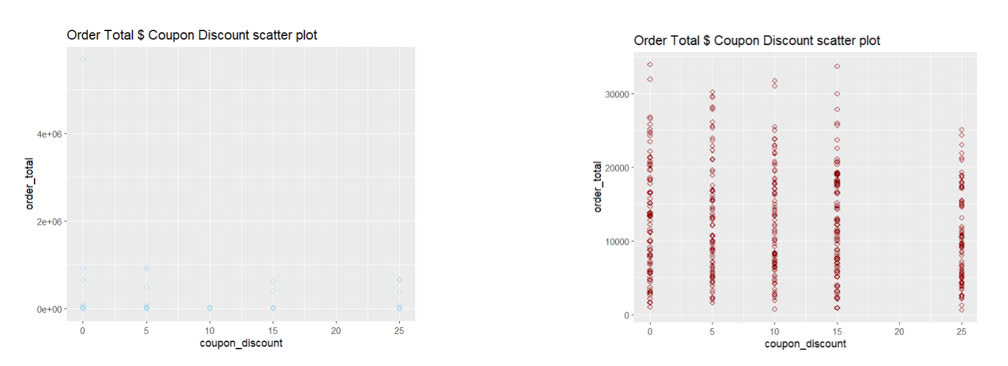
\includegraphics[width=0.8\linewidth]{graphics/bang11.jpg}
    \caption{Hình chưa xóa ngoại lai và đã xóa của coupon\_discount}
    
\end{figure}
\begin{figure}[!htbp]
    \centering
    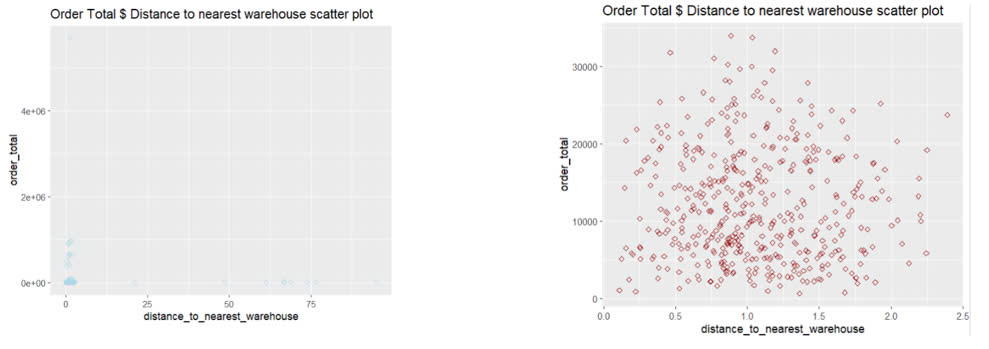
\includegraphics[width=0.8\linewidth]{graphics/bang12.jpg}
    \caption{Hình chưa xóa ngoại lai và đã xóa của distance\_to\_nearest\_warehouse}
 
\end{figure}

\textbf{Nhận xét:} Hai biến order\_price và coupon\_discount là 2 biến có ảnh hưởng tới order\_total hay còn gọi là có quan hệ tuyến tính. Hai biến delivery\_charges và distance\_to\_nearest\_warehouse không có ảnh hưởng tới order\_total hay không có quan hệ tuyến tính.

\subsubsection{Phân tích biến phân loại bằng biểu đồ boxplot}
Ta phân tích biến order\_total theo các biến nearest\_warehouse, season, is\_expedited\_delivery, is\_happy\_customer.
\begin{figure}[!htbp]
    \centering
    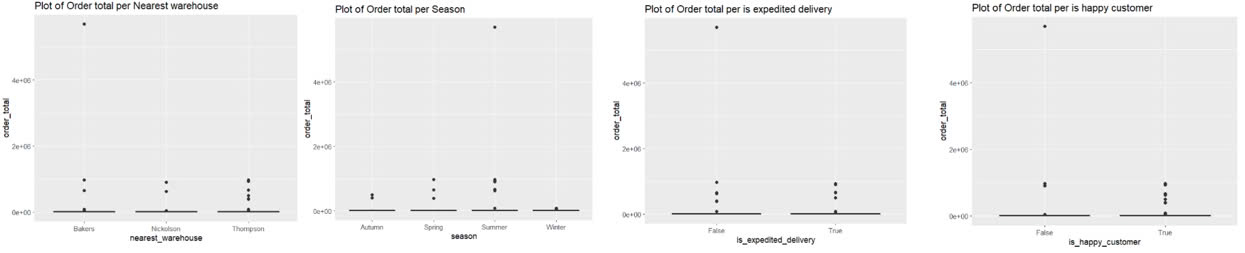
\includegraphics[width=1\linewidth]{graphics/bang13.jpg}
    \caption{Biểu đồ boxplot chưa xóa ngoại lai của các biến phân loại}
\end{figure}

\textbf{Nhận xét:} hình \ref{fig:4.8}.
\begin{itemize}
    \item Cả ba kho hàng (Bakers, Nickolson, Thompson) đều có phân bố tổng đơn hàng tương tự nhau, với các giá trị trung vị (median) gần như ngang bằng.
    \item Phân bố giá trị order\_total khá đồng đều qua các mùa, tuy nhiên mùa Đông có một vài đơn hàng nổi bật với giá trị rất lớn.
    \item Hình thức giao hàng nhanh dường như không có ảnh hưởng rõ rệt đến tổng giá trị đơn hàng trong phần lớn các trường hợp.
    \item Trạng thái hài lòng của khách hàng không tạo ra sự khác biệt lớn trong tổng giá trị đơn hàng, nhưng nhóm khách hàng hài lòng có xu hướng chi tiêu nhiều hơn một chút và có thể thực hiện các đơn hàng có giá trị rất lớn (outliers).
\end{itemize}
\subsection{Bảng tương quan giữa các biến}
Bảng đánh giá tương quan trong đồ thị trên được sử dụng để hiểu rõ mối quan hệ giữa các biến số trong tập dữ liệu.
\pagebreak
\begin{figure}[!htbp]
       \centering
    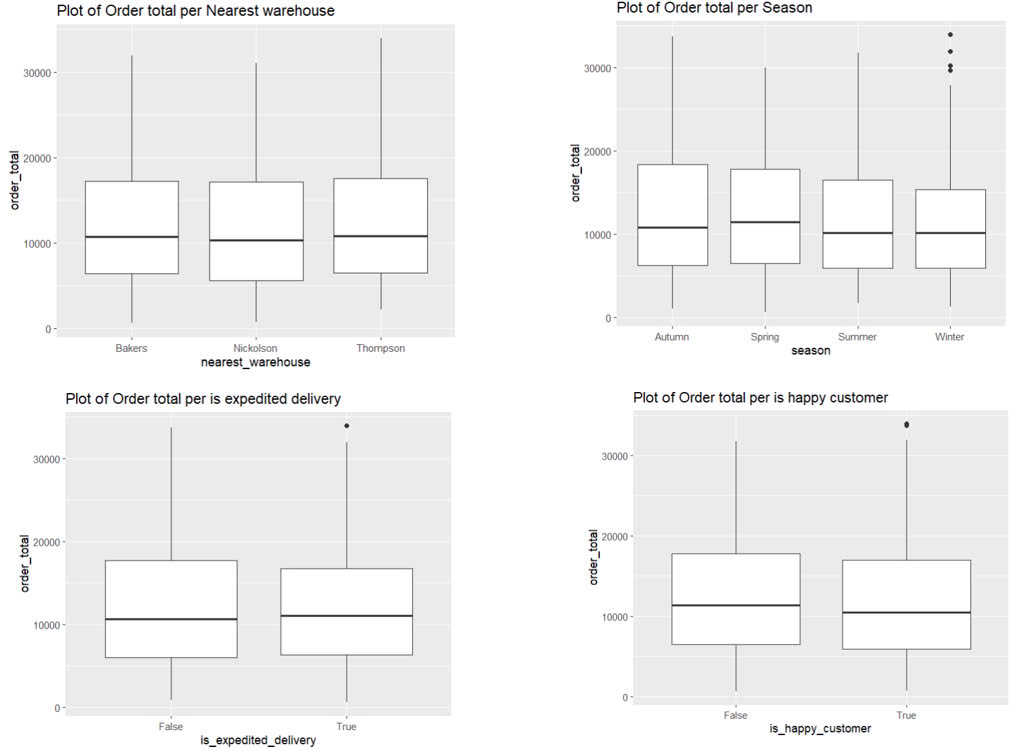
\includegraphics[width=1\linewidth]{graphics/bang14.jpg}
    \caption{Biểu đồ boxplot đã xóa ngoại lai của các biến phân loại}
    \label{fig:4.8}
\end{figure}

\textbf{Nhận Xét:} hình \ref{fig:4.9}
\begin{itemize}
    \item order\_price và order\_total (tương quan: +0.90):
    Đây là mối tương quan dương mạnh. Khi giá trị của order\_price tăng, order\_total cũng tăng mạnh theo và ngược lại. Điều này dễ hiểu vì order\_price là một thành phần chính của order\_total.
    
    \item distance\_to\_nearest\_warehouse và customer\_lat (+0.30):
    Có mối tương quan dương trung bình giữa khoảng cách đến kho hàng và vĩ độ của khách hàng. Điều này có thể ngụ ý rằng vị trí kho hàng có xu hướng gần các khu vực cụ thể về mặt địa lý.
    
    \item distance\_to\_nearest\_warehouse và delivery\_charges (+0.24):
    Mối tương quan dương nhẹ cho thấy khoảng cách đến kho hàng có tác động nhỏ đến chi phí giao hàng. Khoảng cách lớn hơn thường đi kèm với phí giao hàng cao hơn.
    
    \item order\_price và delivery\_charges (+0.02):
    Hầu như không có mối liên hệ giữa giá trị đơn hàng và phí giao hàng. Điều này có thể chỉ ra rằng phí giao hàng không phụ thuộc vào giá trị đơn hàng mà dựa trên các yếu tố khác như khoảng cách hoặc chính sách giao hàng.
    
    \item coupon\_discount với hầu hết các biến khác (gần 0):
    Mức giảm giá từ phiếu coupon không có mối liên hệ đáng kể với bất kỳ biến nào trong tập dữ liệu, kể cả order\_total. Điều này có thể ngụ ý rằng chiến lược giảm giá không ảnh hưởng rõ ràng đến hành vi mua sắm của khách hàng.
\end{itemize}
\begin{figure}[!htbp]
    \centering
    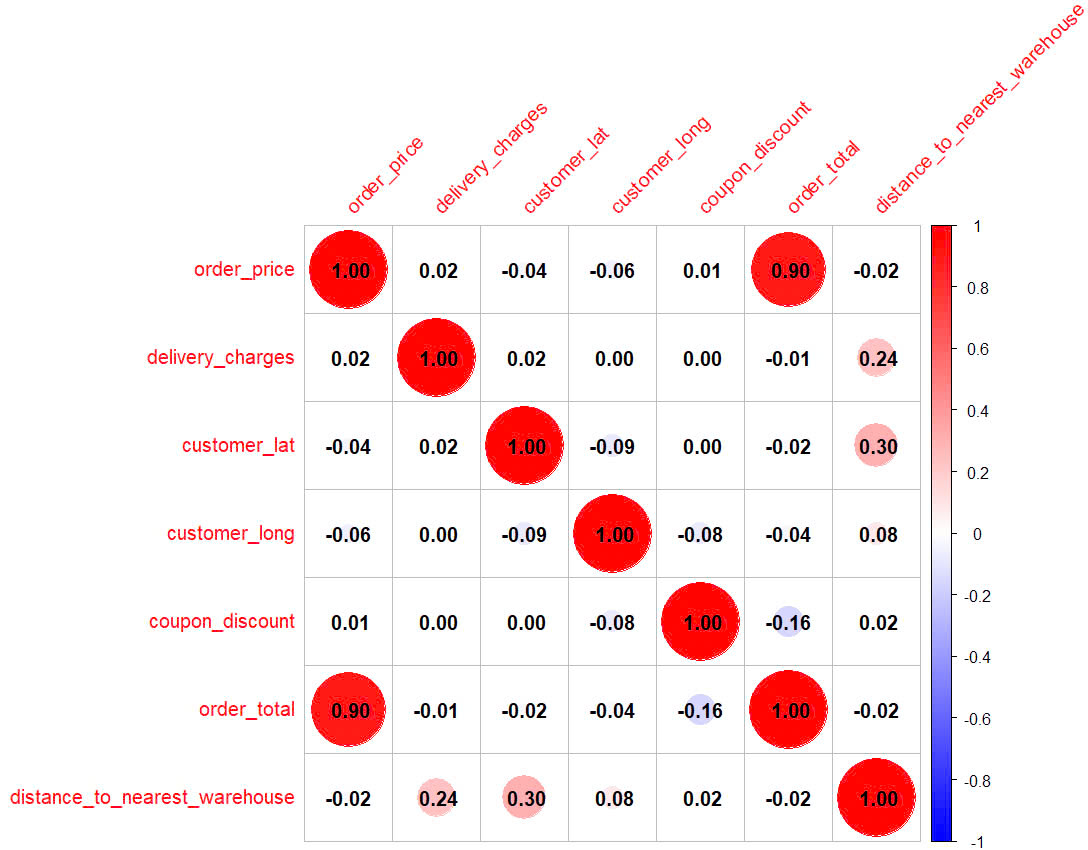
\includegraphics[width=0.8\linewidth]{graphics/tq.jpg}
    \caption{Biểu đồ tương quan của các biến}
    \label{fig:4.9}
\end{figure}